\section{Berechnung von Punkttrajektorien}

\begin{figure*}[bt]\centering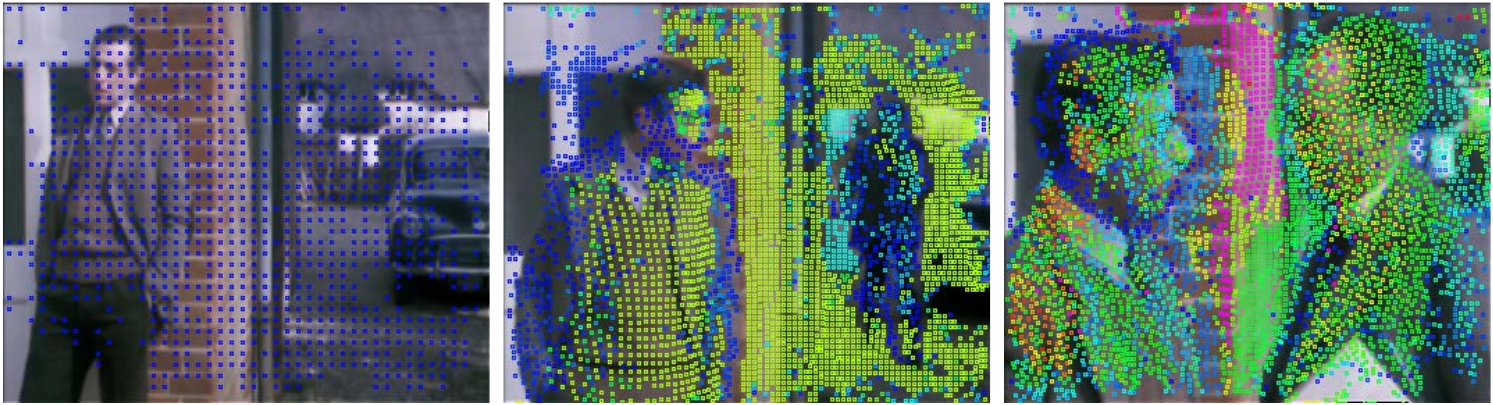
\includegraphics[width=7.0in]{images/trajectories.png}
  \caption{Von links nach rechts: Das erste Frame ursprünglichen Punkt. Sie wurden nur dort initialisiert, wo auch genügend Struktur vorhanden ist.
    Frames 211 und 400 zeigen das Tracking der Punkte. Die Farbe gibt die Dauer des Trackings an (angefangen mit blau als jüngste, über grün, gelb, rot
    und magenta als älteste Punkte).}
  \label{fig:trajectories}
\end{figure*}

Als Grundlage der Trajektorienberechnung dient das von \cite{a001} vorgestellte Verfahren Large Displacement Optical Flow (LDOF).
Dies wird verwendet, um ein optisches Flussfeld $\textbf{w} = (u,v)^T$ zwischen zwei aufeinanderfolgende Bilder einer Videosequenz zu berechnen.

Zunächst wird auf dem ersten Frame des Videos eine Menge von Punkten initialisiert, deren Bewegung auf den darauf folgenden Frames verfolgt werden soll (Abbildung~\ref{fig:trajectories}).
Theoretisch könnte man jedes einzelne Pixel eines Bildes versuchen zu verfolgen, jedoch würde dies zu einem ungemeinen Anstieg der erforderlichen
Rechenkraft führen, zum anderen sind besonders Punkte, die in Bereichen ohne Struktur liegen nur sehr schwer zu verfolgen. Daher werden die Punkte entfernt,
die keine Struktur besitzen, bzw. deren zweiter Eigenwert $\lambda_2$ des Strukturtensors
\begin{equation}
  J_\rho = K_\rho \sum \limits_{k=1}^3 (\nabla I_k)(\nabla I_k)^T
\end{equation}
einen verhältnissmäßig kleinen Wert annimmt. Dabei entspricht $K_p$ einem Gauß-Filter mit Standardabweichung $\rho = 1$ und
$\nabla I_k$ dem Gradient im Farbkanal $k$.

Jeder dieser Punkte kann nun über den zuvor bestimmten optischen Fluss auf das nächste Frame
\begin{equation}
  (x_{t+1}, y_{t+1})^T = (x_t,y_t)^T + (u_t(x_t,y_t), v_t(x_t,y_t))^T
\end{equation}
verfolgt werden. Da der optische Fluss Subpixel-genau arbeitet, ergeben sich für $x$ und $y$ üblicherweise Koordinatenwerte zwischen dem Gitter.
Eine bilinear Interpolation liefert wieder die entsprechenden Punkte auf dem Gitter.

Um die Richtigkeit der Trajektorien zu gewährleisten, muss zuverlässig erkannt werden, wann ein Punkt verdeckt wird und nicht mehr weiter verfolgt werden
kann. Ansonsten würde ein Punkt die Bewegung von zwei unterschiedlichen Objekten beschreiben. Um einen Punkt auf Okklusion zu testen, wird dazu
der Vorwärts- und Rückwärtsfluss überprüft. Diese sollten im nicht verdeckten Fall genau entgegen gerichtet sein:
$ u_t(x_t,y_t) = -\hat{u}_t(x_t + u_t, y_t + v_t) $ und $ v_t(x_t,y_t) = -\hat{v}_t(x_t + u_t, y_t + v_t) $, wobei
$\hat{\textbf{w}}_t := (\hat{u}_t,\hat{v}_t)^T$ dem optischen Fluss von Frame $t+1$ nach $t$ entspricht. Falls diese Bedingung nicht erfüllt sein sollte,
dann wurde der Punkt in $t+1$ entweder verdeckt oder der Fluss wurde nicht richtig bestimmt. Da es jedoch immer zu kleinen Berechnungsfehlern
im optischen Fluss kommen kann, wird für die Überprüfung eine kleine Toleranz zugelassen, die sich linear zur Bewegungsgeschwindigkeit verhält:
\begin{equation}
  | \textbf{w} + \hat{\textbf{w}}|^2 < 0.01 (|\textbf{w}|^2 + |\hat{\textbf{w}}|^2) + 0.5
\end{equation}

Des weiteren werden Punkte an Bewegungskanten nicht weiter verfolgt, da die genaue Schätzung der Grenzen durch den optischen Fluss immer leicht
variiert. Dies kann zu einem ähnlichen Effekt wie bei der Okklusion führen, bei dem ein Punkt plötzlich auf die andere Seite der Grenze fällt
und somit die Bewegung von zwei unterschiedlichen Objekten beschreibt. Um dies zu verhindern, wird ein zusätzliche Bedingung für die korrekte
Verfolgung eingeführt:
\begin{equation}
  |\nabla u|^2 + |\nabla v|^2 > 0.01 |\textbf{w}|^2 + 0.002
\end{equation}

Letztendlich wird noch versucht, die leeren Bereiche des Bildes, die durch Okklusion enstanden sind, wieder zu füllen. Daher werden in jedem neuen Frame
neue Punkte auf die gleiche Weise wie im ersten Bild initialisiert.


\subsection{Segmentierung von Punkttrajektorien}

\begin{figure*}[bt]\centering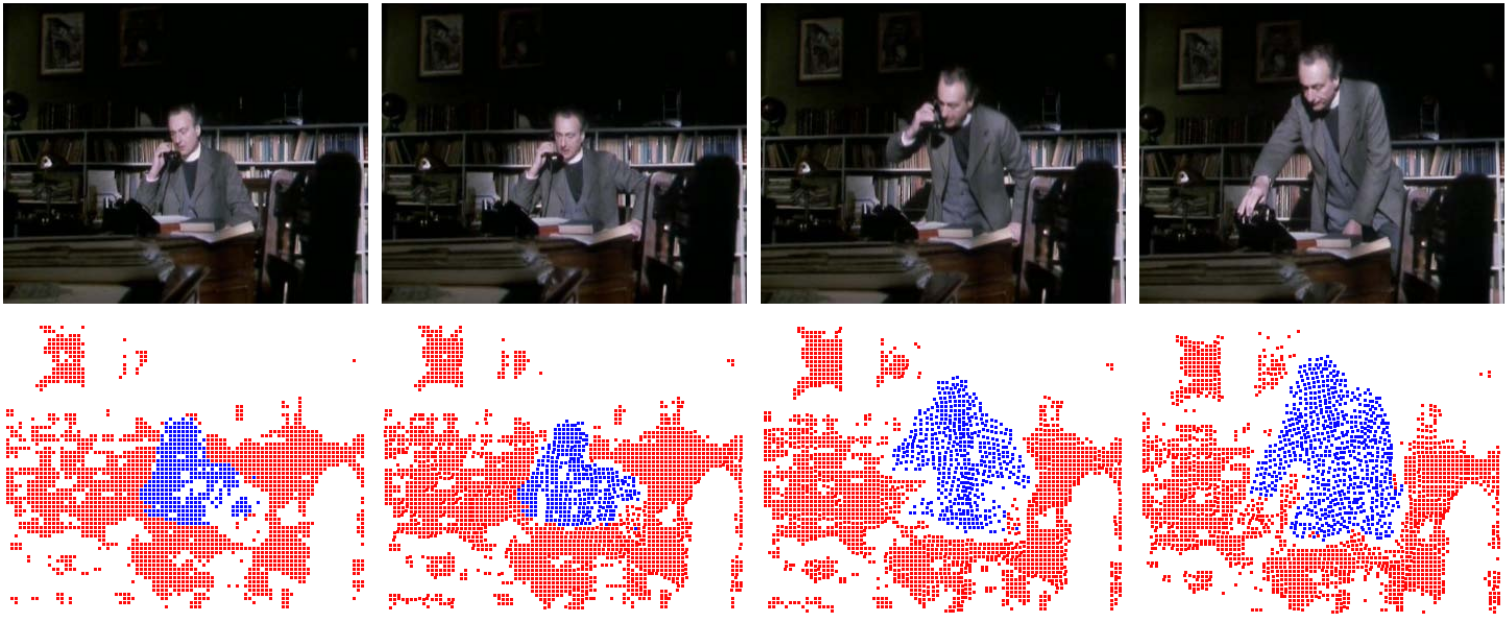
\includegraphics[width=7.0in]{images/motion.png}
  \caption{Frames 0, 30, 50, 80 eines Teils aus dem Film \emph{Miss Marple: Murder at the vicarage}. Bis zu Frame 30 gibt es kaum Bewegung,
  da die Person sitzt. Die meiste Information wird geliefert, sobald sie aufsteht. Mit Hilfe der Langezeit-Verfolgung, ist diese Information
auch im erste Frame verfügbar.}
  \label{fig:motion}
\end{figure*}


Nachdem nun die Punkttrajektorien zur Verfügung stehen, wird das Objektsegmentierungsverfahren von \cite{a001} zum Clustern verwendet.
Wie in Abbildung~\ref{fig:trajectories} zu sehen ist, können diese Trajektorien sich über sehr lange Zeiträume erstrecken, können zeitweise
verdeckt werden oder zu jeder Zeit neue dazukommen. Würden nun nur die Trajektorien ausgewählt werden, die die gesamte Videosequenz abdecken,
würde das Set am Ende sehr klein oder sogar ganz leer sein. Daher wird zum Vergleich eine paarweise Affinität zwischen allen Trajektorien definiert,
die mindestens ein gemeinsames Frame besitzen. Diese Affinitäten definieren dann einen Graphen, auf dem anschließend ein Spectral Clustering Verfahren
angewendet werden kann. Durch diese Transitivität können selbst Trajektorien, die niemals ein gemeinsames Frame besitzen,
dem selben Cluster zugeordnet werden.

Schließlich gilt es noch zu beachten, dass es zu Situationen kommen kann, in denen man zwei Objekte mit gleicher Bewegung nicht von einander unterscheiden
kann. Die tatsächliche Information liegt daher nicht in der gemeinsamen Bewegung, sonderen im Bewegungsunterschied. Sobald also zum Beispiel eine Person
ihre Bewegungsrichtung ändert und diese sich nicht mehr mit der anderen Person gleicht, besitzt man eine genug Daten, um zu wissen, dass diese beiden
Regionen im Bild nicht zusammen gehören (Abbildung~\ref{fig:motion}).

Daraus kann nun eine Distanzmetrik zwischen zwei Trajektorien $A$ und $B$ definierte werden
\begin{equation}
  d^2(A,B) = \mathrm{max}_t d_t^2(A,B),
\end{equation}
an der Stelle, an der der Bewegungsunterschied zwischen zwei Punkten am größten ist. Die Distanz zwischen zwei Punkten zum Zeitpunkt $t$ ist definert als:
\begin{equation}
  d_t^2(A,B) = d_{sp}(A,B) \frac{(u_t^A - u_tt^B)^2 + (v_t^A - v_t^B)^2}{5\sigma_t^2}
\end{equation}
Dabei bezeichneit $d_{sp}(A,B)$ die mittlere, euklidische Distanz von A und B in einem gemeinsame Zeitfenster. Diese räumliche Gewichtung weist
nahen Punkten eine größere Bedeutung zu. $u_t := x_{t+5} - x_t$ und $v_t := y_{t+5} - y_t$ bezeichnet die gemittelte Bewegung eines Punktes über fünf Frames,
was zusätzliche Genauigkeit bietet. $\sigma_t$ schließlich fügt eine Normalisierung der Distanz hinzu
\begin{equation}
  \sigma_t = min_{a\in\{A,B\}} \sum \limits_{t'=1}^5 \sigma(x_{t+t'}^a,y_{t+t'}^a,t+t'),
\end{equation}
wobei $\sigma : \mathbb{R}^3 \rightarrow \mathbb{R}$ die Varianz des lokalen optischen Flusses darstellt. Diese Normalisierung soll sicherstellen, dass
schnelle und langsame Bewegungen gleichermaßen behandelt werden.

Schließlich werden diese Distanzen mittels
\begin{equation}
  w(A,B)= \mathrm{exp}(-\lambda d^2(A,B)), \quad \lambda = 0.1
\end{equation}
in Affinitäten umgewandelt, die dann eine $n \times n$ Matrix $W$ für die gesamte Sequenz bilden, wobei $n$ die Anzahl der Trajektorien ist.

Auf diese Affinitätsmatrix können nun gewöhnliche Clusterverfahren angewendet werden. Die Authoren von \cite{007} stellen jedoch auch
eine anpasste Variante des Spectral Clusterings vor, dass um einen räumlichen Regularisierer erweitert wurde, mit dem Ziel, Übersegmentierungen zu vermeiden.


%%% Local Variables: 
%%% mode: latex
%%% TeX-master: "../main"
%%% End: 
